%HW03.tex
%
% Third Homework for Graduate Algebra
% Frank Sottile
%%%%%%%%%%%%%%%%%%%%%%%%%%%%%%%%%%%%%%%%%%%%%%%%%%%%%%%%%%%%%%%%%%%%%%%
\documentclass[12pt]{article}
\usepackage{multicol,amssymb,amsmath}
\usepackage{colordvi,graphicx}
\headheight=8pt
%
\topmargin=-75pt
\textheight=720pt   \textwidth=560pt
\oddsidemargin=-60pt \evensidemargin=-60pt

\pagestyle{empty}

%%%%%%%%%%%%%%%%%%%%%%%%%%%%%%%%%%%%%%%%%%%%
\newcommand{\CC}{{\mathbb C}}
\newcommand{\KK}{{\mathbb K}}
\newcommand{\NN}{{\mathbb N}}
\newcommand{\QQ}{{\mathbb Q}}
\newcommand{\RR}{{\mathbb R}}
\newcommand{\TT}{{\mathbb T}}
\newcommand{\ZZ}{{\mathbb Z}}

\newcommand{\calA}{{\mathcal A}}
\newcommand{\bfe}{{\bf e}}
\newcommand{\bfi}{{\bf i}}
\newcommand{\bfj}{{\bf j}}

\newcommand{\Hom}{\mbox{Hom}}
\newcommand{\spec}{\mbox{spec}}
\newcommand{\cone}{\mbox{cone}}

\newcommand{\vect}[2]{(\begin{smallmatrix}#1\\#2\end{smallmatrix})}
\newcommand{\msp}{\hspace{8pt}}

\newcommand{\Square}{\raisebox{-2pt}{\includegraphics{images/Square.eps}}}


\def\Color#1#2{\special{color push cmyk #1}#2\special{color pop}}
%\def\Indigo#1{\Color{.42 1. 0. .49}{#1}}
\def\Indigo#1{\Color{1. .95 .05 .4}{#1}}
\def\MyViolet#1{\Color{.6 1. 0. .15}{#1}}


\newcommand{\barsl}{\noindent\begin{minipage}[t]{590pt}
\Indigo{\rule{590pt}{1.2pt}}\vspace{-5.7mm}\\
\MyViolet{\rule{590pt}{1.2pt}}\vspace{-5.7mm}\\
\Blue{\rule{590pt}{1.2pt}}\vspace{-5.7mm}\\
\Green{\rule{590pt}{1.2pt}}\vspace{-5.7mm}\\
\Yellow{\rule{590pt}{1.2pt}}\vspace{-5.7mm}\\
\Orange{\rule{590pt}{1.2pt}}\vspace{-5.7mm}\\
\Red{\rule{590pt}{1.2pt}}\bigskip
\end{minipage}}


\newcommand{\barsn}{\noindent\begin{minipage}[t]{590pt}
\Indigo{\rule{590pt}{1.1pt}}\vspace{-4.5mm}\\
\MyViolet{\rule{590pt}{1.1pt}}\vspace{-4.5mm}\\
\Blue{\rule{590pt}{1.1pt}}\vspace{-4.5mm}\\
\Green{\rule{590pt}{1.1pt}}\vspace{-4.5mm}\\
\Yellow{\rule{590pt}{1.1pt}}\vspace{-4.5mm}\\
\Orange{\rule{590pt}{1.1pt}}\vspace{-4.5mm}\\
\Red{\rule{590pt}{1.1pt}}\bigskip
\end{minipage}}

\def\demph#1{\Maroon{{\sl #1}}}
\def\defcolor#1{\Maroon{#1}}

\begin{document}
\LARGE 
\noindent
Algebra \ \ Autumn 2023\vspace{1pt}\\
Frank Sottile\vspace{1pt}\\
\Large 6 September 2023 \hfill
\sf
 Third Homework\makebox[40pt][l]{\ }
\large\vspace{10pt}

\noindent
Write your answers neatly, in complete sentences.  
I highly recommend recopying your work before handing it in.
Correct and crisp proofs are greatly appreciated; oftentimes your work can be shortened and made clearer.

\barsl

\noindent\Maroon{{\large\sf Hand in for the grader Monday 11  September:}}
\bigskip


\begin{enumerate}
\setcounter{enumi}{11}


%%%%%%%%%%%%%%%%%%%%%%%%%%%%%%%%%%%%%%%%%%%%%%%%%%%%%%%%%%%%%%%%%%%%%%%%%%%%%%%%%%%%%%%%%%%%%%%%%%%%
%Autumn 2017, 2023
\item Let $x_1,\dotsc,x_n$ be variables.
   Prove the following \demph{Vandermonde identity}\newline
   $\det(x_i^{j-1})_{i,j=1}^n=\prod_{1\leq a<b\leq n}(x_b-x_a)$.
   For example, 
\[
   \det\left(\begin{matrix}1&1&1&1\vspace{-5pt}\\x_1&x_2&x_3&x_4
          \\x_1^2&x_2^2&x_3^2&x_4^2\\x_1^3&x_2^3&x_3^3&x_4^3\end{matrix}\right)\
     =\ (x_2-x_1)(x_3-x_1)(x_4-x_1)(x_3-x_2)(x_4-x_2)(x_4-x_3)\,.
\]
%%%%%%%%%%%%%%%%%%%%%%%%%%%%%%%%%%%%%%%%%%%%%%%%%%%%%%%%%%%%%%%%%%%%%%%%%%%%%%%%%%%%%%%%%%%%%%%%%%%%  

 
%%%%%%%%%%%%%%%%%%%%%%%%%%%%%%%%%%%%%%%%%%%%%%%%%%%%%%%%%%%%%%%%%%%%%%%%%%%%%%%%%%%%%%%%%%%%%%%%%%%%
%Autumn 2013  chenged for Autumn 2023
\item %List all of the elements of $S_4$ in cycle notation.
  What is the maximum order of an element of $S_4$?
      Use this to prove that $D_{24}$, the dihedral group of order 24, is not isomorphic to
      $S_4$.
%%%%%%%%%%%%%%%%%%%%%%%%%%%%%%%%%%%%%%%%%%%%%%%%%%%%%%%%%%%%%%%%%%%%%%%%%%%%%%%%%%%%%%%%%%%%%%%%%%%%  

%%%%%%%%%%%%%%%%%%%%%%%%%%%%%%%%%%%%%%%%%%%%%%%%%%%%%%%%%%%%%%%%%%%%%%%%%%%%%%%%%%%%%%%%%%%%%%%%%%%%
%Autumn 2013 and 2023
\item Let $SL_2(\ZZ_3)$ be the group of $2\times 2$ matrices of determinant $1$ 
   with entries in the field $\ZZ_3$ with three elements.
  Show that  $SL_2(\ZZ_3)$ has order 24, and that it is not isomorphic to $S_4$.
  Is it isomorphic to $D_{24}$?
%%%%%%%%%%%%%%%%%%%%%%%%%%%%%%%%%%%%%%%%%%%%%%%%%%%%%%%%%%%%%%%%%%%%%%%%%%%%%%%%%%%%%%%%%%%%%%%%%%%%  


%%%%%%%%%%%%%%%%%%%%%%%%%%%%%%%%%%%%%%%%%%%%%%%%%%%%%%%%%%%%%%%%%%%%%%%%%%%%%%%%%%%%%%%%%%%%%%%%%%%%
%Autumn 2017 and 2023
\item     
   Let $m\geq 2$ be an integer.
   Set $\defcolor{\ZZ^*_m}:=\{ k\in \ZZ_m \mid \gcd(k,m)=1\}$.
    These are the cosets of integers that are relatively prime to $m$.
  \begin{enumerate}

   \item  Show that $\ZZ^*_m$ is the set of generators of the cyclic group $\ZZ_m$.
      \vspace{-2pt}

   \item  Show that $\ZZ^*_m$ is a group under multiplication modulo $m$.
         Define $\defcolor{\phi(m)}:=|\ZZ^*_m|$, the order of this group.
          This is Euler's \demph{totient function}, also called Euler's $\phi$-function.\vspace{-2pt}

   \item  Deduce Euler's Theorem.
          If $\gcd(a,m)=1$, then $a^{\phi(m)} \equiv 1\ \mod m$. \newline
           (That is, $m$ divides $a^{\phi(m)} -1$, equivalently, $a^{\phi(m)}=1$ as elements of $\ZZ_m$.)
            \vspace{-2pt}

   \item  Let $p$ be a prime number and show that $\phi(p)=p-1$.
         
          Determine $\phi(p^n)$, where $p$ is a prime and $n>0$ is an integer.

          Show that $\phi$ is multiplicative; if $a,b\in\NN$ are relatively prime, ($\gcd(a,b)=1$), then 
           $\phi(ab)=\phi(a)\cdot\phi(b)$.

          Deduce a formula for $\phi(m)$ in terms of the factorization of $m$ into a product of powers of distinct
          primes.
          Express this in terms of $m$ and its distinct prime divisors.
      \vspace{-2pt}

   \item   Deduce  Fermat's Little Theorem from the last part.
           If $p$ is any prime number and $a\in\ZZ$, then $a^p\equiv a\ \mod p$.
         
\end{enumerate}
%%%%%%%%%%%%%%%%%%%%%%%%%%%%%%%%%%%%%%%%%%%%%%%%%%%%%%%%%%%%%%%%%%%%%%%%%%%%%%%%%%%%%%%%%%%%%%%%%%%%  

      
\end{enumerate}
%%%%%%%%%%%%%%%%%%%%%%%%%%%%%%%%%%%%%%%%%%%%%%%%%%%%%%%%%%%%%%%%%%%%%%%%%%%%%%%%%%%%%%%%%%%%%%%%%%%%

\end{document}
